\usetheme[numbering=fraction]{metropolis}

\metroset{block=fill}

\usepackage[dvipsnames]{xcolor}

\usepackage{booktabs}

\usepackage{fancyvrb}
\fvset{listparameters=\setlength{\topsep}{0pt}\setlength{\partopsep}{0pt}}

\usepackage{csquotes}
\setquotestyle{british}

\usepackage{graphicx}
\graphicspath{ {../../images/} }

\usepackage{pgfplots}
\usetikzlibrary{positioning,calc,external}
%\tikzexternalize[prefix=figures/] 

\usepackage{crysymb}

\renewcommand*{\arraystretch}{1.2}

\usepackage{soul}
\usepackage[en-GB]{datetime2}
\DTMlangsetup[en-GB]{ord=omit}

\usetikzlibrary{positioning,calc}
\graphicspath{ {../../images/} }

\title[Short version of title]{ICS0026 Cryptography}
\subtitle{Hash functions, KDFs \& MACs}
\date{\DTMdate{2024-03-05}}
\author%
{%
    {Taaniel Kraavi}\\
    \textit{\footnotesize Guest Lecturer}
}
\institute%
{%
    \textit{IT College}\\
    \textit{Tallinn University of Technology}
}

\begin{document}
\begin{frame}
  \titlepage
\end{frame}

\begin{frame}{Hash functions}
  \pause
  A map from arbitrary sized data to fixed-size values.
  \begin{itemize}[<+(1)->]
    \item $h:\{0,1\}^* \to \{0,1\}^n$
    \item Some functions provide variable-length output
    \item Values are called \emph{hashes} or \emph{digests}
    \item Deterministic
  \end{itemize}

  \vspace*{1em}

  \pause
  A good hash function:
  \begin{itemize}[<+(1)->]
    \item fast
    \item minimal collisions
  \end{itemize}
\end{frame}

\begin{frame}{Pigeonhole principle}
  \pause
  If $n$ items are put into $m$ containers, with $n > m$, then at least one container must contain more than one item.

  \vspace*{1em}

  \pause
  \begin{center}
    \includegraphics[height=150px]{pigeonhole}
  \end{center}
\end{frame}

\begin{frame}{Hash collisions}
  By the pigeonhole principle, hashing is susceptible to collisions.
  \begin{itemize}[<+(1)->]
    \item Different inputs have the same hash
    \item $h(x_1) = h(x_2), x_1 \neq x_2$
  \end{itemize}

  \vspace*{1em}

  \pause
  Consequences:
  \begin{itemize}[<+(1)->]
    \item `General computing': bad performance (e.g. indexing)
    \item Cryptography: loss of integrity and/or security
  \end{itemize}

  \vspace*{1em}

  \pause
  Not all hash functions provide `strong' integrity guarantees!
\end{frame}

\begin{frame}{Cryptographic hash functions (CHF)}
  A \emph{cryptographic hash function} must additionally satisfy:
  \begin{itemize}[<+(1)->]
    \item Collision resistance (infeasible to find any)
    \item (First) preimage resistance (one-wayness)
    \item Second preimage resistance
    \item Avalanche effect
    \item Uniform output distribution
  \end{itemize}
\end{frame}

\begin{frame}{Different resistances}
  Collision resistance:
  \begin{itemize}[<+(1)->]
    \item Find any two distinct inputs with the same hashes
    \item Find any $x, y$ with $x \neq y$ s.t. $h(x) = h(y)$
  \end{itemize}

  \pause
  (First) preimage resistance:
  \begin{itemize}[<+(1)->]
    \item Given a hash, find the data that produces this hash
    \item Given $h(x)$, find some $x$
  \end{itemize}

  \pause
  Second preimage resistance:
  \begin{itemize}[<+(1)->]
    \item Given an input, find another input that produces the same hash
    \item Given $x$, find $y \neq x$ s.t. $h(x) = h(y)$
  \end{itemize}
\end{frame}

\begin{frame}{Security level}
  Collision resistance:
  \begin{itemize}[<+(1)->]
    \item $n/2$ for $n$-bit hashes (birthday problem)
    \item $n/3$ with quantum computers (disputed)
  \end{itemize}

  \vspace*{1em}

  \pause
  Preimage resistance (first \& second):
  \begin{itemize}[<+(1)->]
    \item $n$ for $n$-bit hashes
    \item $n/2$ with quantum computers
  \end{itemize}
\end{frame}

\begin{frame}{Different resistances}
  Collision resistance $\implies$ second preimage resistance.
  \begin{itemize}[<+(1)->]
    \item Implies first preimage resistance only if input space $\gg$ output space
    \item 2\textsuperscript{nd} preimage resistance:
    \begin{itemize}
      \item weaker assumption
      \item harder problem
    \end{itemize}
    \item 2\textsuperscript{nd} preimage resistance not enough for a `general' case
    \item In addition, it should be hard to find similar hashes
  \end{itemize}

  \vspace*{1em}

  \pause
  Collision \& pre-image resistance are not everything:
  \begin{itemize}[<+(1)->]
    \item Attacks due to constructions may exist
    \item Length extension attack
  \end{itemize}
\end{frame}

\begin{frame}{Similar hashes}
  \pause
  How closely do you check your hashes?
  \begin{center}
    \includegraphics[width=\textwidth]{hashsimil}
  \end{center}
  \vfill
  {\scriptsize\url{https://www.da.vidbuchanan.co.uk/blog/colliding-secure-hashes.html}}
\end{frame}

\begin{frame}[fragile]{Drunken bishops}
  \begin{columns}[onlytextwidth]
    \begin{column}{0.6\textwidth}
      \pause
      Drunken bishops algorithm:
      \begin{itemize}[<+(1)->]
        \item OpenSSH fingerprint visualisation algorithm
        \item ASCII random art
        \item A more reliable visual check
      \end{itemize}
    \end{column}
    \begin{column}{0.3\textwidth}
      \begin{Verbatim}[fontsize=\scriptsize]
+--[ED25519 256]--+
|             ..  |
|           .  +. |
|          + .o .o|
|         = =.. .o|
|        S =.+.=..|
|       o O E.+...|
|      . . B.O  ..|
|       .oo.Oo= ..|
|      .. o*=+oo  |
+----[SHA256]-----+
      \end{Verbatim}
    \end{column}
  \end{columns}

  \vfill

  \pause
  For critical applications, always check hashes programmatically!
\end{frame}

\begin{frame}{Avalanche effect}
  An ideal cryptographic hash function should behave like a random function.
  \begin{itemize}[<+(1)->]
    \item Changing just a single input should re-randomise the output
    \item Flip $50\%$ bits (on average)
    \item Random oracle model (ROM) (does not hold in practice)
  \end{itemize}

  \vspace*{1em}

  \pause
  Example:
  \begin{itemize}
    \item {\small\texttt{md5sum(0x80) = 8d39dd7eef115ea6975446ef4082951f}}
    \item {\small\texttt{md5sum(0x81) = cd25041f9f36811b04ab3015805fe816}}
    \pause\item $83/128$ bits changed
  \end{itemize}
\end{frame}

\begin{frame}{CHF use cases}
  CHFs are a fundamental primitive in cryptography:
  \begin{columns}
    \begin{column}{0.4\textwidth}
      \begin{itemize}[<+(1)->]
        \item Integrity assertion
        \item Key derivation
        \item Message authentication
      \end{itemize}
    \end{column}
    \begin{column}{0.4\textwidth}
      \begin{itemize}[<+(1)->]
        \item CSPRNGs
        \item Digital signatures
        \item Commitments
      \end{itemize}
    \end{column}
  \end{columns}

  \vspace*{1.5em}
  \pause
  Notable use cases:
  \begin{columns}
    \begin{column}{0.4\textwidth}
      \begin{itemize}[<+(1)->]
        \item Proof-of-work (e.g. Bitcoin)
        \item Digital fingerprinting \& fuzzy hashing
      \end{itemize}
    \end{column}
    \begin{column}{0.4\textwidth}
      \begin{itemize}[<+(1)->]
        \item Password storage\textsuperscript{*}
        \item Nothing-up-my-sleeve constructions
      \end{itemize}
    \end{column}
  \end{columns}

  \vspace*{1.5em}
  \pause
  Many more use cases exist (also non-infosec related).
\end{frame}

\begin{frame}{What CHFs are not}
  CHFs are not suitable for encryption:
  \begin{itemize}[<+(1)->]
    \item hashes cannot be `decrypted'
    \item there is no secret key
    \item keyed hash functions: MACs not encryption
  \end{itemize}
\end{frame}

\begin{frame}{What CHFs are not}
  CHFs are not suitable for protecting passwords:
  \begin{itemize}[<+(1)->]
    \item hash functions should be fast to compute
    \item passwords should be slow to brute force
    \item use a KDF designed for passwords instead
  \end{itemize}
\end{frame}

\begin{frame}{What CHFs are not}
  CHFs are not suitable for anonymisation/pseudonymisation:
  \begin{itemize}[<+(1)->]
    \item hash the data and check membership
    \item smaller input spaces are easily pre-computed (e.g. EE ID codes)
    \item you cannot do lookups if you salt the data
  \end{itemize}
\end{frame}

\begin{frame}{Some sus functions}
  Well known hash functions you should not use:
  \begin{itemize}[<+(1)->]
    \item MD5: collisions can be found in seconds
    \item SHA-1: collision \href{https://shattered.io}{\textit{demonstrated}}
  \end{itemize}
\end{frame}

\begin{frame}{Some good functions}
  Hash functions to use:
  \begin{itemize}[<+(1)->]
    \item SHA-2 family
    \begin{itemize}
      \item SHA-224, SHA-256, SHA-384, SHA-512, SHA-512/224, SHA-512/256
      \item Be mindful of length-extension attacks
    \end{itemize}
    \item SHA-3 family (Keccak)
    \begin{itemize}
      \item SHA3-224, SHA3-256, SHA3-384, SHA3-512
      \item SHAKE128, SHAKE256 (variable length output)
    \end{itemize}
    \item BLAKE functions
    \begin{itemize}
      \item BLAKE (SHA-3 finalist), BLAKE2, BLAKE3
      \item Each succeeds the previous
    \end{itemize}
  \end{itemize}
\end{frame}

\begin{frame}{Length extension attacks}
  Given $H(m_1)$ and $\lvert m_1\rvert$, an adversary might compute $H(m_1 || m_2)$ for some $m_2$.
  \begin{itemize}[<+(1)->]
    \item Do not use LE-vulnerable functions for message authentication codes!
    \item Always think whether the attack is a concern!
  \end{itemize}

  \vspace*{1em}

  \pause
  Vulnerable are:
  \begin{itemize}[<+(1)->]
    \item Hash functions based on Merkle-Damgård construction (iterative)
    \item E.g. MD5, SHA-1, non-truncated SHA-2
    \begin{itemize}
      \item SHA-256, SHA-512 but not SHA-384, SHA-512/256
      \item SHA-224 is truncated, but is weak against LE (32 bits of security)
    \end{itemize}
  \end{itemize}

  \pause
  {\scriptsize\url{https://github.com/iagox86/hash_extender} for a PoC}
\end{frame}

\begin{frame}{SHA-2}
  Secure Hash Algorithm 2
  \begin{itemize}[<+(1)->]
    \item Designed by the NSA
    \item Published in 2001
    \item \href{https://csrc.nist.gov/pubs/fips/180-4/upd1/final}{FIPS 180-4 (Secure Hash Standard)}
    \item Merkle-Damgård construction (like SHA-1 before it)
    \item Multiple rounds
    \begin{itemize}
      \item Attacks exist against fewer rounds
    \end{itemize}
  \end{itemize}
\end{frame}

\begin{frame}{SHA-3}
  Secure Hash Algorithm 3
  \begin{itemize}[<+(1)->]
    \item NIST hash function competition (announced 2007)
    \item Need for an alternative construction (to complement SHS)
    \item Published in 2016: won by Keccak
    \item \href{https://csrc.nist.gov/pubs/fips/202/final}{FIPS 202}
    \item Sponge construction (not vulnerable to LE)
    \item Variable length output variants (SHAKE128 \& SHAKE256)
  \end{itemize}
\end{frame}

\begin{frame}{Hash-based structures}
  Hash chains:
  \begin{itemize}[<+(1)->]
    \item Link data with the previous element (linked list)
    \item Any modification to chain elements voids the subsequent chain
    \item The most recent element must be monitored
  \end{itemize}

  \pause
  Hash trees (Merkle trees):
  \begin{itemize}[<+(1)->]
    \item Improvement to the linear nature of the chain
    \item Link elements in a tree structure (e.g. binary tree)
    \item Verify trail using intermediate nodes
    \item The root node must be monitored
  \end{itemize}
\end{frame}

\begin{frame}{Hash chain}
  \begin{center}
    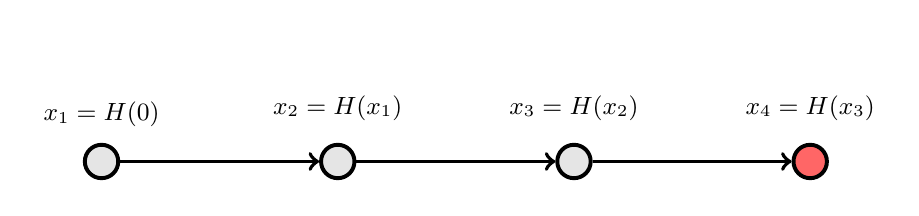
\begin{tikzpicture}
      [every node/.style={fill=gray!20,draw=black,circle,line width=0.5mm,inner sep=1.5mm}]
      \node[label={[yshift=-6mm]\small $x_1 = H(0)$}] (x1) at (0, 0) {};
      \node[label={[yshift=-6mm]\small $x_2 = H(x_1)$}] (x2) at (3, 0) {};
      \node[label={[yshift=-6mm]\small $x_3 = H(x_2)$}] (x3) at (6, 0) {};
      \node[fill=red!60,label={[yshift=-6mm]\small $x_4 = H(x_3)$}] (x4) at (9, 0) {};

      \draw[->,line width=0.5mm] (x1) -- (x2);
      \draw[->,line width=0.5mm] (x2) -- (x3);
      \draw[->,line width=0.5mm] (x3) -- (x4);
    \end{tikzpicture}
  \end{center}

  Link nodes with hashes:
  \begin{itemize}
    \item 1\textsuperscript{st} node: $x_1 = H(0)$
    \item 2\textsuperscript{nd} node: $x_2 = H(x_1) = H\bigl(H(0)\bigr)$
    \item \dots
    \item i\textsuperscript{th} node: $x_i = H(x_{i-1}) = H\Bigl(H\bigl(\dots H(0)\dots\bigr)\Bigr)$
  \end{itemize}
\end{frame}

\begin{frame}{(Binary) Merkle tree}
  \vspace*{-3em}
  \begin{center}
    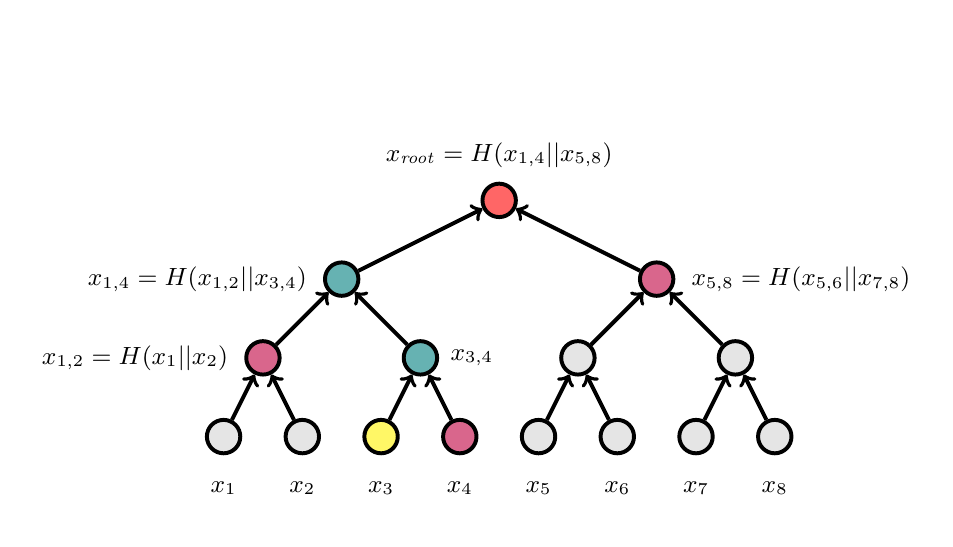
\begin{tikzpicture}
      [level distance=10mm,
      every node/.style={fill=red!60,draw=black,circle,line width=0.5mm,inner sep=1.5mm},
      edge from parent/.style={<-,draw},
      level 1/.style={sibling distance=40mm,line width=0.5mm,nodes={fill=gray!20}},
      level 2/.style={sibling distance=20mm,nodes={fill=gray!20}},
      level 3/.style={sibling distance=10mm,nodes={fill=gray!20}}]
     \node[label={[yshift=-13mm]north:\small $x_{\mathit{root}}=H(x_{1,4}||x_{5,8})$}] {}
        child {node[label={left:\small $x_{1,4}=H(x_{1,2}||x_{3, 4})$},fill=teal!60] {}
          child {node[label={left:\small $x_{1,2}=H(x_1||x_2)$},fill=purple!60] {}
            child {node[label=south:{\small $x_1$}] {}}
            child {node[label=south:{\small $x_2$}] {}}
          }
          child {node[label={[xshift=-1mm]right:\small $x_{3,4}$},fill=teal!60] {}
            child {node[label=south:{\small $x_3$},fill=yellow!60] {}}
            child {node[label=south:{\small $x_4$},fill=purple!60] {}}
          }
        }
        child {node[label={right:\small $x_{5,8}=H(x_{5,6}||x_{7,8})$},fill=purple!60] {}
          child {node {}
            child {node[label=south:{\small $x_5$}] {}}
            child {node[label=south:{\small $x_6$}] {}}
          }
          child {node {}
            child {node[label=south:{\small $x_7$}] {}}
            child {node[label=south:{\small $x_8$}] {}}
          }
        };
    \end{tikzpicture}
  \end{center}
  Knowing node $x_3$, we can verify the path to the root given only:
  \[
    H(x_4), H(x_{1,2}), H(x_{5,8}), H(x_{\mathit{root}})
  \]
\end{frame}

\begin{frame}{Widely witnessed evidence}
  \begin{center}
    \includegraphics[width=0.8\textwidth]{guardtime_root}\\
    The Guardtime Merkle root published in a newspaper.
  \end{center}

  \pause
  {\scriptsize\url{https://x.com/Guardtime/status/1759897737212899612?s=20} most recent root}
\end{frame}

\begin{frame}{KDFs}
  Key derivation functions:
  \begin{itemize}[<+(1)->]
    \item Derive one or many keys from secret data
    \begin{itemize}
      \item obtain keys of a required format
      \item e.g. hybrid encryption (cryptographic KDF)
    \end{itemize}
    \item Stretch and/or strengthen keys from the input data:
    \begin{itemize}
      \item user-provided passwords: short and low entropy
      \item protect passwords (password `hashing')
      \item increase brute-force resistance
      \item e.g. securely store passwords in \texttt{/etc/shadow}
      \item e.g. symmetric key from a password (password-based KDF)
    \end{itemize}
  \end{itemize}

  \vspace*{1em}

  \pause
  Use the right KDF for the right task!
  \begin{itemize}
    \pause\item Password hashing $\to$ key stretching: do not use CHFs!
  \end{itemize}
\end{frame}

\begin{frame}{Key stretching}

  \pause
  Introduce randomness with a \emph{salt}:
  \begin{itemize}[<+(1)->]
    \item similar to a nonce/IV: \emph{always} use but \emph{do not re-use}
    \item use \emph{before} hashing to change the output
    \item store the salt alongside the hash, it is \emph{not secret}
    \item prevents pre-computation attacks (e.g. rainbow tables) for long-enough salts
  \end{itemize}
  
  \pause
  Increase execution time/resources needed:
  \begin{itemize}[<+(1)->]
    \item e.g. iterative hashing: $H(H(H(\dots H(H(\mathit{password}))\dots)))$
    \begin{itemize}
      \item different techniques exist, e.g. by increasing memory usage
      \item no computational shortcuts must be known
    \end{itemize}
    \item slows down brute-force (e.g. dictionary attacks)
    \item different use-cases: different parameters (social media login vs. FDE)
    \item use at least the recommended minimum params (KDF-dependent)
  \end{itemize}

\end{frame}

\begin{frame}[fragile]{Salted password validation}
  To validate a provided password:
  \begin{enumerate}[<+(1)->]
    \item look up the salted password with an identifier (e.g. username)
    \item hash the provided password with the stored salt
    \item compare the result with the stored result
    \item accept or reject
  \end{enumerate}

  \vspace*{1em}

  \pause
  Example of a salted hash (argon2id):
  \vspace*{-1em}
  \begin{center}
    \texttt{\$argon2id\$v=19\${\color{Melon}m=19456,t=2,p=1}\${\color{CadetBlue}bXlzYWx0IDop}\${\color{PineGreen}16E7QlHDtnMnvUsXDPtqKA}}\\
    \texttt{%
    \ \ \ \ \ \ \ \ \ \ \ \ \ \ \ \ %
    \ {\color{Melon}params}\ \ \ \ \ %
    \ \ \ \ \ {\color{CadetBlue}salt}\ \ \ \ \ %
    \ \ \ \ \ \ {\color{PineGreen}pwd hash}%
    \ \ \ \ \ \ \ }
  \end{center}
\end{frame}

\begin{frame}{Peppering}
  A pepper is a secret data used to protect passwords:
  \begin{itemize}[<+(1)->]
    \item is shared among all passwords in a database
    \item secret, and not stored with the password
    \begin{itemize}
      \item store on a HSM or a vault
      \item if the DB can be breached, what else can...
    \end{itemize}
    \item trickier to use for questionable benefit
    \begin{itemize}
      \item good salting will protect the passwords
      \item increases the complexity for yourself
      \item lose the pepper = credentials are void
    \end{itemize}
  \end{itemize}

  \pause
  Peppering can work for your personal passwords:
  \begin{itemize}[<+(1)->]
    \item use for critical passwords in your password manager
    \item manually enter the prefix/suffix
  \end{itemize}
\end{frame}

\begin{frame}{What to use for password hashing?}
  NIST strikes again:
  \begin{itemize}[<+(1)->]
    \item Password Hashing Competition (2013)
    \item Winner: Argon2
  \end{itemize}

  \vspace*{1em}

  \pause
  OWASP password storage cheat sheet (\href{https://cheatsheetseries.owasp.org/cheatsheets/Password_Storage_Cheat_Sheet.html}{\textit{link}}):
  \begin{enumerate}[<+(1)->]
    \item Use Argon2id whenever possible (not Argon2d or Argon2i)
    \item \texttt{scrypt} if Argon2id is not available
    \item \texttt{bcrypt} for legacy systems
    \item PBKDF2 if FIPS-compliance is needed
  \end{enumerate}

  \pause
  Suggested parameters in \href{https://datatracker.ietf.org/doc/html/rfc9106\#name-parameter-choice}{RFC9106} and the OWASP cheat sheet.
\end{frame}

\begin{frame}{Message authentication codes (MACs)}
  Authenticate and verify a message's integrity:
  \begin{itemize}[<+(1)->]
    \item authentication \emph{tag} requires a shared secret to compute
    \item any party with the secret can create valid MACs
    \item it should be infeasible to compute a valid MAC without the secret
    \item if the message is tampered with, the tag should not validate
  \end{itemize}
\end{frame}

\begin{frame}{Naive construction}
  Naive construction: SHA-256 with a secret key (keyed hashing)
  \begin{itemize}[<+(1)->]
    \item Set the tag $t = \mathsf{SHA\text{-}256}(k||m)$
    \item Recipient verifies $t$ by recomputing the keyed hash
    \item Length extension attacks! (and other subtle attacks)
  \end{itemize}

  \vspace*{1em}

  \pause
  Do not build your own MACs!
  \begin{itemize}[<+(1)->]
    \item Use special-purpose MAC algorithms.
    \item Use parameters suggested by reputable sources (will be homework ;))
  \end{itemize}
\end{frame}

\begin{frame}{What to use}
  First, check what the documentation/standard recommends for your use case.

  \vspace*{1em}

  \pause
  In a standalone setting, use
  \begin{itemize}[<+(1)->]
    \item HMAC (\href{https://csrc.nist.gov/pubs/fips/198-1/final}{FIPS 198-1}): hash-based message authentication code
    \item KMAC (\href{https://csrc.nist.gov/pubs/sp/800/185/final}{NIST SP 800-185}): Keccak MAC
  \end{itemize}
\end{frame}

\begin{frame}{What to use}
  For authenticated encryption, stick with the following combos:
  \begin{enumerate}[<+(1)->]
    \item XChaCha20-Poly1305
    \item AES-GCM-SIV (nonce reuse resistance)
    \item ChaCha20-Poly1305
    \item AES-GCM
    \item AES-CTR/AES-CBC + HMAC-SHA2 (only if none of the above is possible)
  \end{enumerate}

  \vspace*{1em}

  \pause
  Encrypt first, then MAC the ciphertext: Encrypt-then-MAC (EtM).

  \vspace*{1em}

  \pause
  Never reuse nonces under a same key!
\end{frame}

\begin{frame}{Using MACs}
  You should almost always use a MAC!
  \begin{itemize}[<+(1)->]
    \item Not needed if solid authentication is integrated into the scheme.
    \item Encrypt-then-MAC (EtM): authenticates the ciphertext.
    \item Do not use the same key for encryption and the MAC.
  \end{itemize}

  \vspace*{1em}

  \pause
  MACs work with symmetric ciphers and in hybrid systems:
  \begin{itemize}[<+(1)->]
    \item The public-key `equivalent' is digital signatures
    \item We will cover signatures next week
    \item A signature scheme can replace a MAC in \emph{some} contexts.
  \end{itemize}
\end{frame}

\end{document}
